\part{Ejercicio 4}
\section{Introducción}
	El objetivo es realizar dos circuitos, el circuito derivador e integrador, que como sus nombres indican se encargan de mostrar a la salida la derivada  o integral respectivamente de su señal de entrada.
	Como se indica por consigna se utilizó el amplificador operacional LM833 y el valor comercial más cercano al pedido tanto de resistencia como de capacitor, estos son $R \ = \ 39k \Omega$ y $C \ = \ 2.7 nF$.

%$R=40k\Omega -> 39k \Omega$
%$C = 2.5 nF -> 2.7 nF$
\section{Cálculo de $\frac{V_{out}}{V_{in}}$}
Mientras en uno de los dos circuitos la resistencia y la impedancia tienen una disposición, para el otro se intercambian de lugar, por lo que los siguientes cálculos se realizaron con impedancias $Z_1$ y $Z_2 $ como se muestra en la Figura \ref{fig:circconz1z2} y luego se reemplazó con el valor correspondiente al circuito al que se hizo mención.
\begin{figure}[H]
\centering
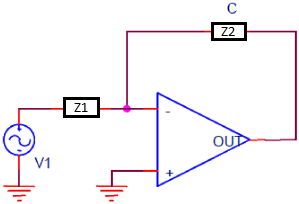
\includegraphics[scale=0.5]{../Ex4/circconz1z2.png}
\caption{Circuito con impedancias Z1 y Z2}
\label{fig:circconz1z2}
\end{figure}

\subsection{Idealidad}
Se consideró $V^+\,=V^-$ , entonces:
\begin{equation}
	H(s) = \dfrac{V_{out}}{V_{in}} = - \dfrac{Z_2}{Z_1} = G_I
	\label{eq:gananciaideal}
\end{equation}
$G_I$: Ganancia Ideal.

\subsection{Con $A_{vol}$ finito}
Si dejamos de lado el caso ideal y consideramos que la ganancia no es infinita, se consigue el siguiente sistema de ecuaciones considerando aún que la impedancia del operacional es infinita:

\begin{equation}
\begin{cases}
V_{out} = A_{vol} \ (V^+ - V^-) = - A_{vol} \ V^- \\ V_{out} - V^- = i \ Z_2 \\ V_{out} - V_{in} = i \ (Z_1+Z_2) 
\end{cases} 
\end{equation}

\begin{equation}
H(s) = - \dfrac{Z_2}{Z_1} \dfrac{1}{1+\dfrac{1+\dfrac{Z_2}{Z_1}}{A_{vol}}}
= -
\dfrac{A_{vol} \ Z_2}{Z_2 + Z_1 (A_{vol} +1)}
\end{equation}

Si $A_{vol} \longrightarrow \infty$ obtenemos la expresión para $H(s)$ vista para el caso ideal.
También se puede escribir $H(s)$ en función de $G_I$:
\begin{equation}
H(s) = \dfrac{A_{vol} \, Z_2 \, G_I}{A_{vol} + 1 - G_I} 
\end{equation}

Viendo el datasheet del amplificador operacional utilizado se notó que $90 \ dB< A_{vol} < 110 \ dB$ a condiciones normales de temperatura ($25 \ ºC$) y alimentando con $\pm 15 \ V$.

\subsection{Con $A_{vol}(w)$ con polo dominante}
\begin{equation}
H(s) = - \dfrac{\dfrac{A_{vol}}{1+\dfrac{s}{w_p}} \ Z_2}{Z_2 + Z_1 \left(\dfrac{A_{vol}}{1+\dfrac{s}{w_p}} +1 \right)} 
=
-\dfrac{A_{vol} \ Z_2}{(Z_1+Z_2) \left(\dfrac{s}{w_p}+1 \right)+ A_{vol} \ Z_1}
\end{equation}

%-\frac{\mathrm{A_{vol}} \ Z_{2}}{\left(\dfrac{s}{\mathrm{w_p}}+1\right)\,\left(Z_{2}+Z_{1}\,\left(\dfrac{\mathrm{A_{vol}}}{\dfrac{s}{\mathrm{w_p}}+1}+1\right)\right)}

%= - \dfrac{Z_2 \ \left( \dfrac{A_{vol} \ w_p}{s}  + 1 \right)}{Z_2 + Z_1 \ \left( \dfrac{A_{vol} \ w_p}{s}  + 1 \right)}%
En este caso también se aplica que si $A_{vol} \longrightarrow \infty$ obtenemos la expresión para $H(s)$ vista para el caso ideal.
El datasheet nos informa que el valor de \textit{BWP} del \textit{LM833} es de $15 \ MHz$.
Si se tiene en cuenta la ecuación (\ref{eqwp}) podemos obtener el valor de $w_p$.
\begin{equation}\label{eqwp}
BWP = A_{vol} \ . \ w_p \Rightarrow w_p= 2 \ . \pi \ \frac{BWP}{A_{vol}}= 2 \ . \ \pi \ \frac{15x10^6}{10^{\frac{110}{20}}} = 2 \ . \ \pi \ . \ 47,4342 \ Hz
\end{equation}















\section{Circuito Derivador}
En este caso al circuito visto en la Figura \ref{fig:circconz1z2} se le reemplazo $Z_1$ por un capacitor y $Z_2$ por una resistencia como puede verse en la Figura \ref{fig:circuitoderivador}. En este caso $Z_1=\dfrac{1}{s \, C}$ y $Z_2= R$.
\begin{figure}[H]
\centering
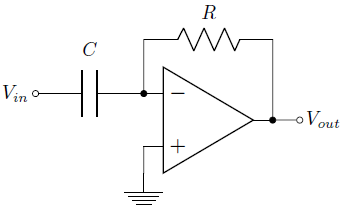
\includegraphics[scale=0.5]{../Ex4/circuitoderivador.png}
\caption{Circuito derivador}
\label{fig:circuitoderivador}
\end{figure}

Se utilizó además $\mathrm{A_{vol}}=110$.

\subsection{Ganancia Ideal}
Reemplazando los valores de $Z_1$ y $Z_2$ por los mencionados en la subsección anterior en la Ecuación \ref{eq:gananciaideal} se obtiene:
\begin{equation}
G_I=H_{ideal}(s)= - \ R \,C \,s
\end{equation}


\begin{center}
	\begin{figure}[H]	
	\makebox[\textwidth]{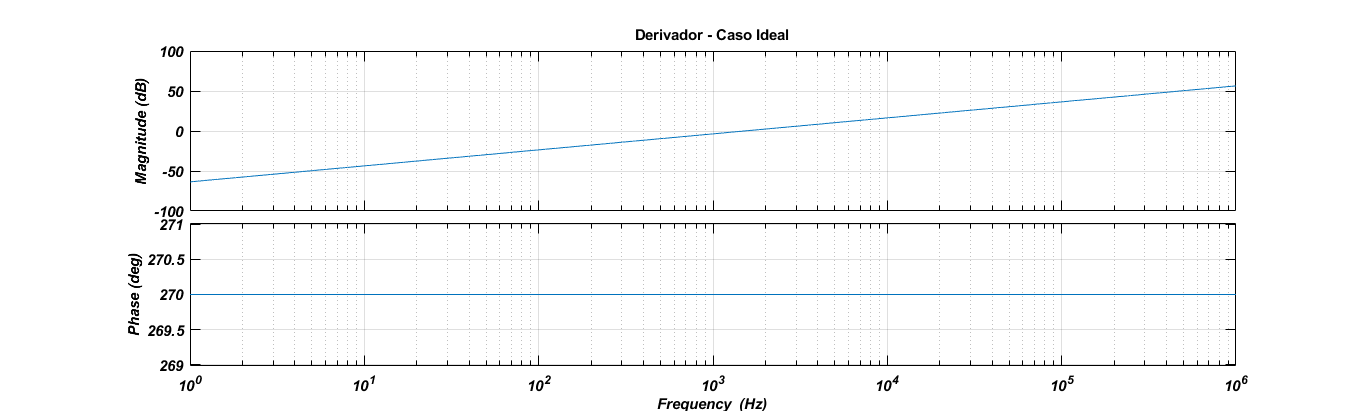
\includegraphics[width=\paperwidth]{../Ex4/Derivador-CasoIdeal.png}}
	\caption{Ganancia para el caso ideal del derivador}
	\label{fig:avolidealderivador}
	\end{figure}
\end{center}

Si se realiza la antitransformada recordando que $H(s)= \dfrac{V_{out}}{V_{in}}$ obtenemos:
\begin{equation} 
v_{out} (t) = - \ R \,C \, \dfrac{\partial v_{in}(t)}{\partial t}
\end{equation}
Donde se observa que la función a la salida es la derivada de la función a la entrada multiplicada por una constante que es $- R\,C$. También al observar la función transferencia se puede notar un desfasaje de $-90º$ y la presencia de un cero simple en $f \sim 1.5 \,kHz$, lo que otorga una ganancia de $20 \, dB$ por década.

\subsection{$\mathrm{A_{vol}}$ finito}
\begin{equation}
H(s) = - \dfrac{A_{vol} \,C\,R\,s}{A_{vol} + C \,R \,s +1 } 
= -
\left( \dfrac{A_{vol} \,R \,C}{A_{vol} + 1} \right) \, \dfrac{s}{ \left( \dfrac{s}{\dfrac {A_{vol} +1}{R \,C}} \right) + 1}
\end{equation}

Se observa que se agrega en este caso un polo en $f = \dfrac{1}{2 \,\pi} \, \dfrac {A_{vol} +1}{R \,C} \sim 478 \, MHz $, notando así en la Figura \ref{avolfinitoderivador} que la ganancia comienza a tomar un valor constante  cerca de este valor. Si se toma que $A_0 >>> 1$ se obtiene $H(s)=- \dfrac{A_{vol} \,C\,R\,s}{A_{vol} + C \,R \,s}$, teniendo así un comportamiento similar al de un filtro pasa altos que explica porque al llegar a la frecuencia de corte la magnitud adopta un valor constante.

La fase tiene un cambio de $-90º$ lento que comienza aproximadamente a los $50 \, MHz$ y termina de cambiar alrededor de los $5 \,GHz$, pasando así de $-90º$ a $-180º$.

Mientras se trabaje a menores valores de frecuencia que $50 \, MHz$ para así no apreciar cambios en la magnitud o la fase, se puede decir que el comportamiento del circuito no se ve afectado y que se comporta como el ideal. 

\begin{figure}[H]
	\begin{center}
		\makebox[\textwidth]{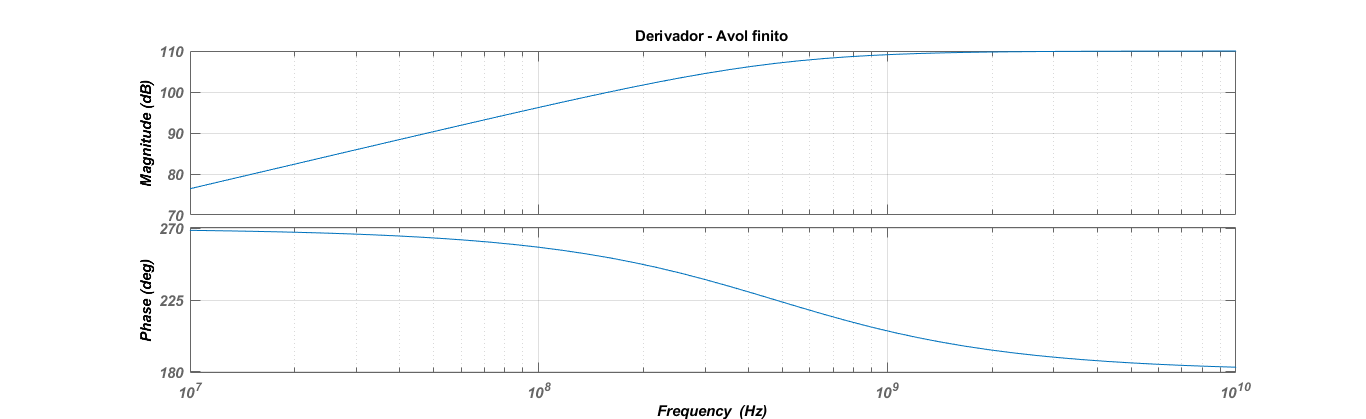
\includegraphics[width=\paperwidth]{../Ex4/Derivador-AvolfinitoBodeAutomatico.png}}
		\caption{Ganancia para el caso con $A_{vol}$ finito del derivador}
		\label{avolfinitoderivador}
	\end{center}
\end{figure}

\subsection{$\mathrm{A{vol}(w)}$ con polo dominante}

\begin{equation}
H(s) = - \left( \dfrac{A_{vol} \,C \,R}{A_{vol} + 1} \right) \, \dfrac{s}{ \dfrac{s^2}{\dfrac{(A_{vol}+1)}{C \,R}} + \dfrac{1+ C \,R \,w_p}{(A_{vol} + 1) \,w_p} \,s + 1} 
\end{equation}

En este tercer caso se observa que hay un polo de segundo orden en $f_0 = \dfrac{1}{2 \,\pi} \sqrt{\dfrac{(A_{vol}+1)}{C \,R} \ w_p} \sim 150 \ kHz$.

\begin{figure}[H]
	\begin{center}
		\makebox[\textwidth]{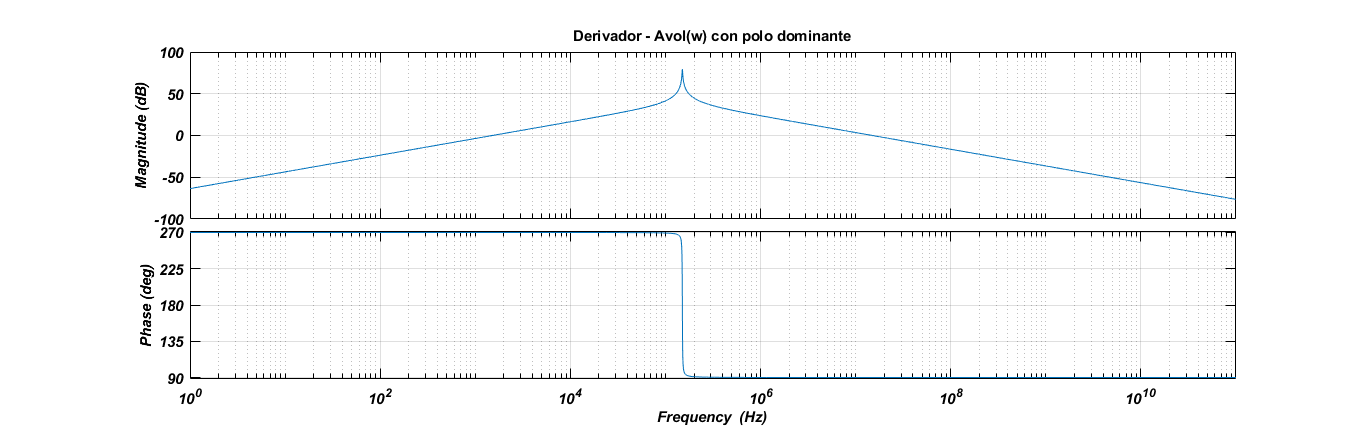
\includegraphics[width=\paperwidth]{../Ex4/Derivador-Avol(w)conpolodominante.png}}
		\caption{Ganancia para el caso con $A_{vol}(w)$ con polo dominante del derivador}
		\label{avolpolodominantederivador}
	\end{center}
\end{figure}

A partir de los $100 \ kHz$ se puede notar que comienza a afectar el polo dominante como un sobrepico en la amplitud y un cambio rápido de $-180º$, cambiando así de $-90º$ a $90º$.

\subsection{Comparación de los 3 casos}	\label{sub:comparaciondelos3casos}
\begin{figure}[H]
	\begin{center}
		\makebox[\textwidth]{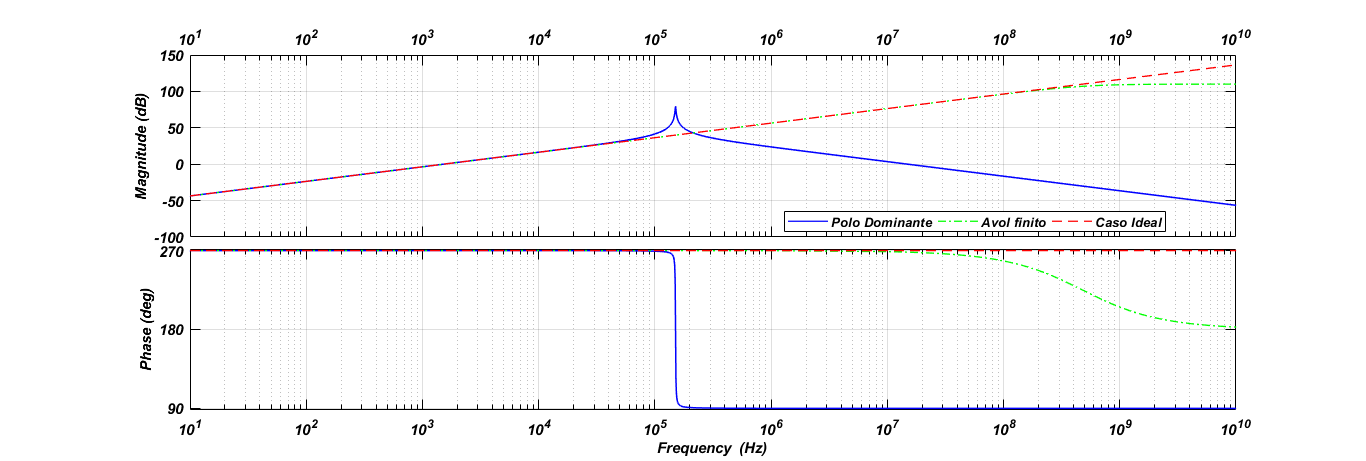
\includegraphics[width=\paperwidth]{../Ex4/BodesSuperpuestos.png}}
		\caption{Superposición de los tres casos}
		\label{fig:comparacion3avolderivador}
	\end{center}
\end{figure}

Viendo el gráfico se notó que a frecuencias menores a aproximadamente $80 \ kHz$ tanto la amplitud como la fase de las tres funciones se comportan de forma idéntica, por lo que si se trabaja con frecuencias menores a $80 \ kHz$ el circuito debe cumplir con el propósito de su diseño, el de derivar.

\subsection{Simulación LTSpice}
\begin{figure}[H]
	\begin{center}
		\makebox[\textwidth]{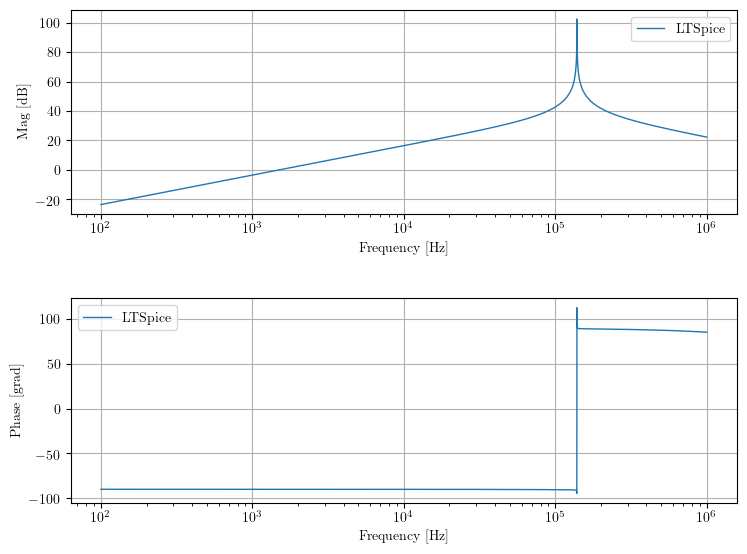
\includegraphics[width=0.6\paperwidth]{../Ex4/BodeDerivadorLTSpiceGUI.png}}
		\caption{Bode de la simulación en LTSpice}
		\label{fig:simulacionderivador}
	\end{center}
\end{figure}

\subsection{Medición}
\begin{figure}[H]
	\begin{center}
		\makebox[\textwidth]{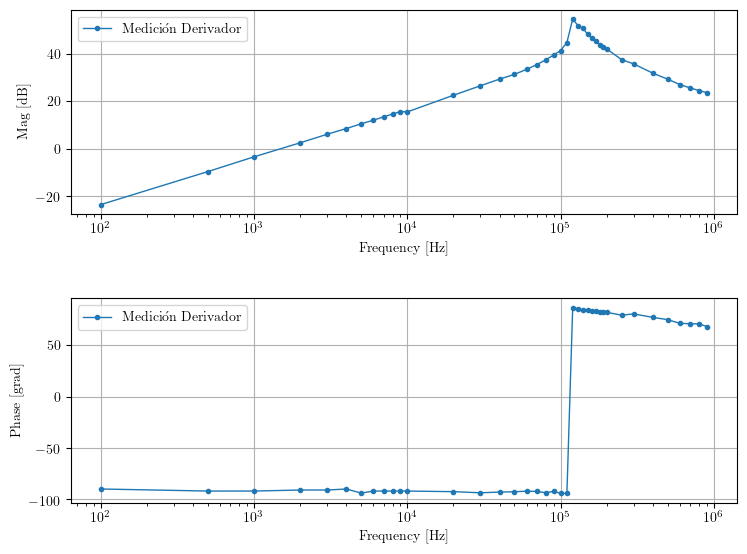
\includegraphics[width=0.6\paperwidth]{../Ex4/BodeDerivadorMEdidoGUI.png}}
		\caption{Bode medido}
		\label{fig:medicionderivador}
	\end{center}
\end{figure}


Como la ganancia es muy alta en las frecuencias cercanas al sobrepico, no se pudo tomar más medidas para tener una mayor precisión ya que para que la tensión de salida no saturara habría que alimentarla con valores de tensión de entrada muy pequeños, lo cual no es posible con la instrumentación con la que se cuenta ya que a pesar de que el generador de señales con el que se cuenta puede llegar hasta un mínimo de $20 \, V_{pp}$, se estaría trabajando en el orden del ruido del osciloscopio y la medición no sería correcta.

\subsection{Medición vs. simulación vs. teórico}
\begin{figure}[H]
	\begin{center}
		\makebox[\textwidth]{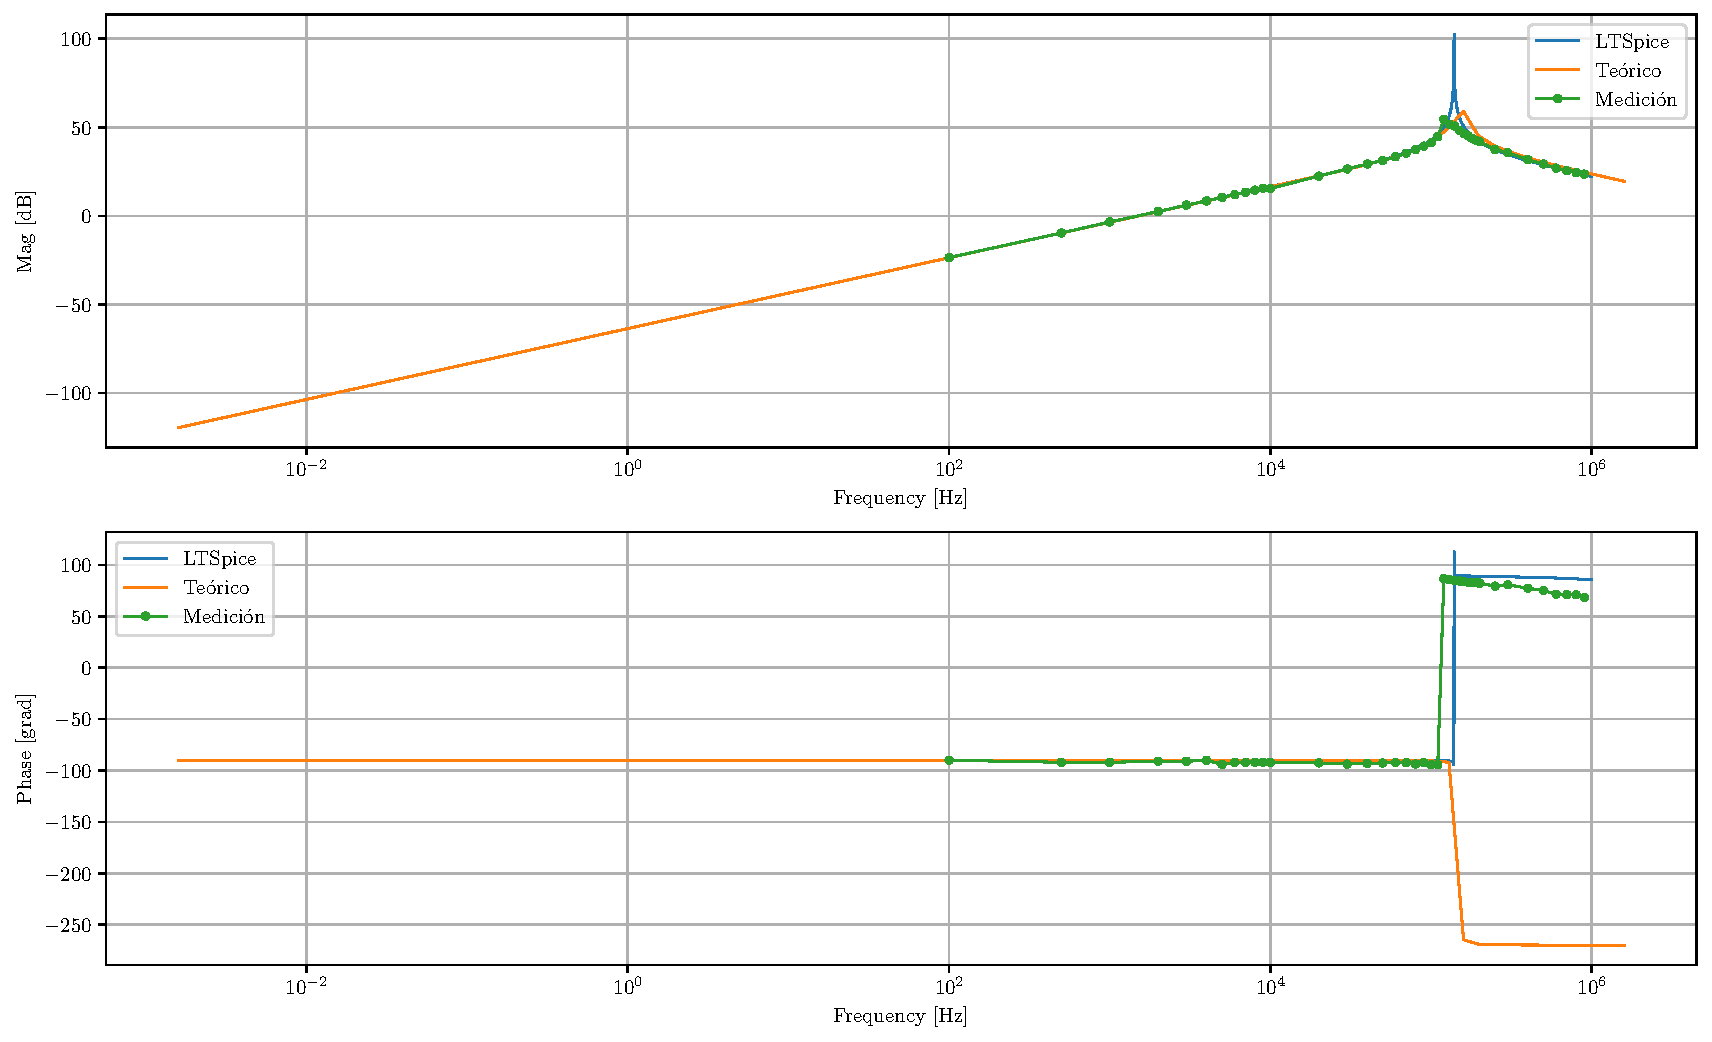
\includegraphics[width=\paperwidth]{../Ex4/BodesSuperpuestosDERivadorARREGLARFASE.pdf}}
		\caption{Superposición de bodes para el circuito derivador}
		\label{fig:superposiciontrescasos}
	\end{center}
\end{figure}

Como se observa en la Figura \ref{fig:superposiciontrescasos} el circuito fabricado se comporta de igual manera que el simulado en LTSpice y el teórico hasta aproximadamente $110 \, kHz$ que es donde se tiene un cambio de fase abrupto a esta frecuencia y no alrededor de los $140 \, kHz$. Notar que al comportarse de igual manera que el teórico hasta esa frecuencia, sigue siendo válido lo dicho en la Sección \ref{sub:comparaciondelos3casos} sobre su rango de utilización.

\subsection{Comportamiento ante señales no senoidales}

\begin{figure}[H]
	\begin{center}
		\makebox[\textwidth]{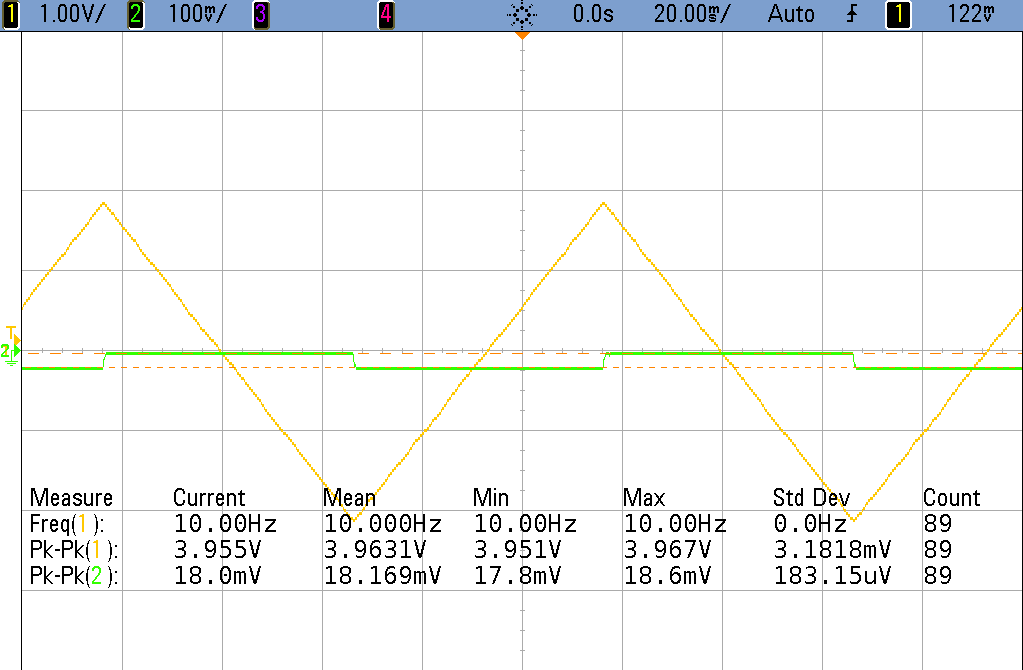
\includegraphics[width=0.8\textwidth]{../Ex4/DerivTriang10HzNOComp.png}}
		\caption{Derivada de una señal triangular a $10 \, Hz$}
		\label{fig:derivtriangNOcomp10Hz}
	\end{center}
\end{figure}

Se puede observar que el circuito deriva la señal de entrada ya que muestra a la salida en verde una señal cuadrada que efectivamente es la derivada de la señal de entrada triangular amarilla. Notar que la señal cuadrada es positiva en la parte en la cual la señal triangular desciende y esto se debe a que la ganancia se encuentra multiplicada por un factor negativo como se vio en las secciones anteriores donde se calculo la ganancia.

\begin{figure}[H]
	\begin{center}
		\makebox[\textwidth]{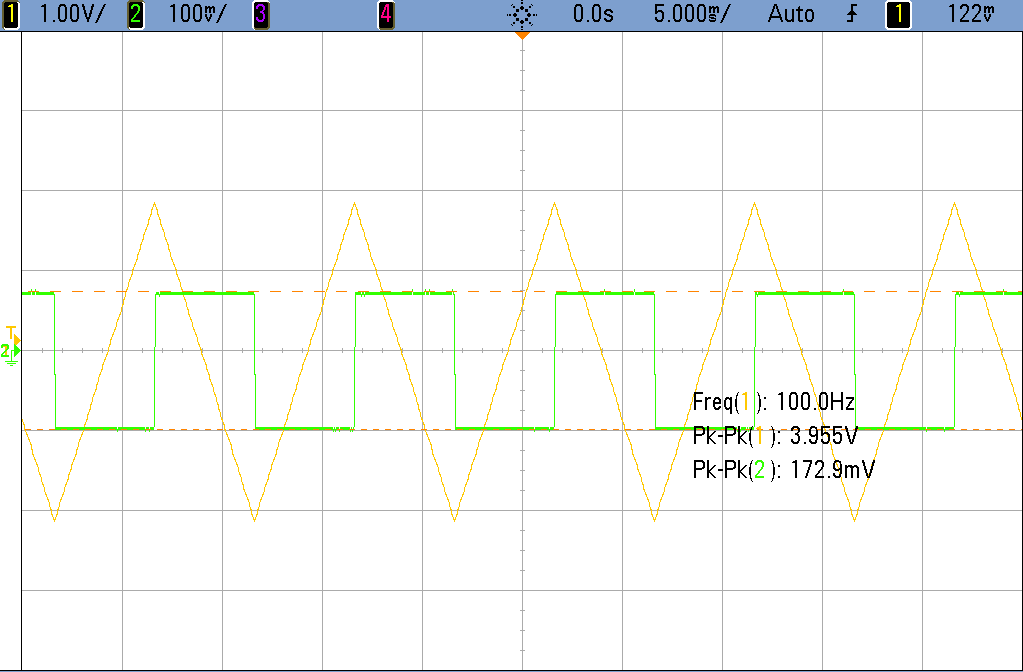
\includegraphics[width=0.8\textwidth]{../Ex4/DerivTriang100HzNOComp.png}}
		\caption{Derivada de una señal triangular a $100 \, Hz$}
		\label{fig:derivtriangNOcomp100Hz}
	\end{center}
\end{figure}

Se puede notar si se compara la Figura \ref{fig:derivtriangNOcomp100Hz} con la Figura \ref{fig:derivtriangNOcomp10Hz} que al aumentar la frecuencia ha aumentado el valor de la tensión en la salida.

\begin{figure}[H]
	\begin{center}
		\makebox[\textwidth]{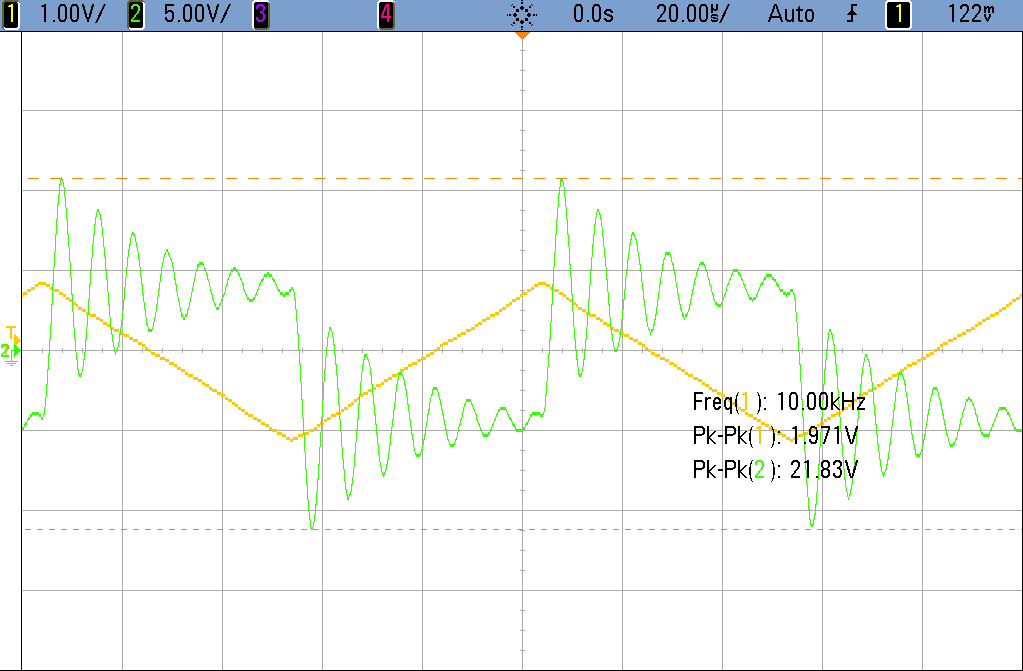
\includegraphics[width=0.8\textwidth]{../Ex4/DerivTriang10kHzNOComp.png}}
		\caption{Derivada de una señal triangular a $10 \, kHz$}
		\label{fig:derivtriangNOcomp10kHz}
	\end{center}
\end{figure}

La salida oscila hasta estabilizarse y esto se deba al hecho de que estamos ante un sistema subamortiguado, siendo así ya que los polos del sistema son complejos conjugados.

\begin{figure}[H]
	\begin{center}
		\makebox[\textwidth]{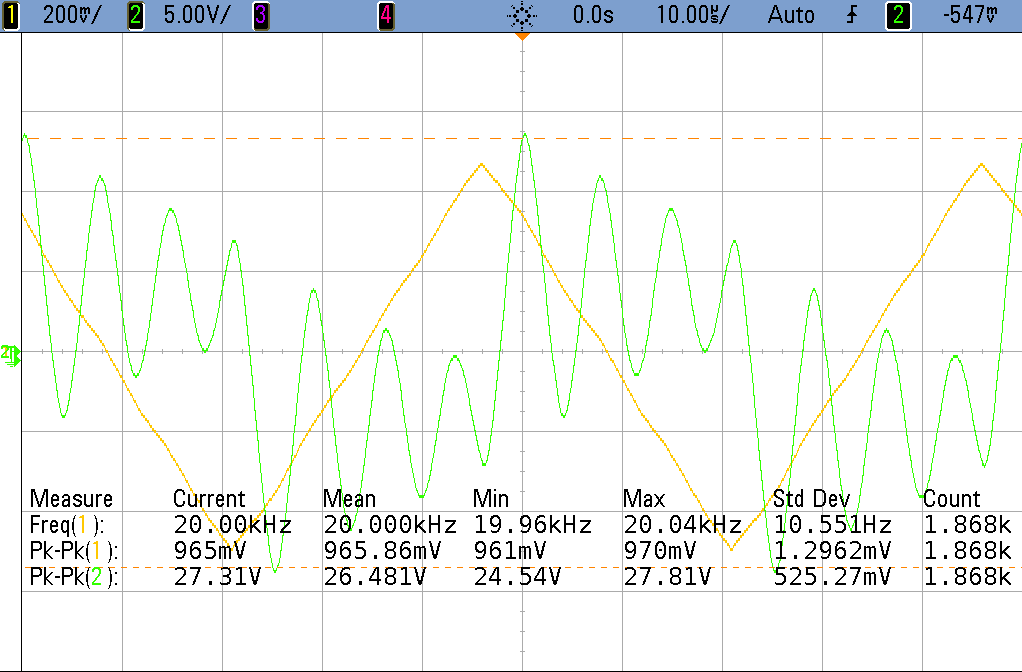
\includegraphics[width=0.8\textwidth]{../Ex4/DerivTriang20kHzNOComp.png}}
		\caption{Derivada de una señal triangular a $20 \, kHz$}
		\label{fig:derivtriangNOcomp20kHz}
	\end{center}
\end{figure}

A esta frecuencia el circuito ya no tiene el tiempo suficiente para estabilizarse y se observa solamente la respuesta transitoria.

\subsection{Impedancia de entrada}
Se utilizó el analizador de impedancias para poder realizar las mediciones que procedieron a volcarse en la Figura \ref{fig:zinsuperDERivador} donde se superponen la impedancia de entrada simulada con LTSpice y la medida.


\begin{figure}[H]
	\begin{center}
		\makebox[\textwidth]{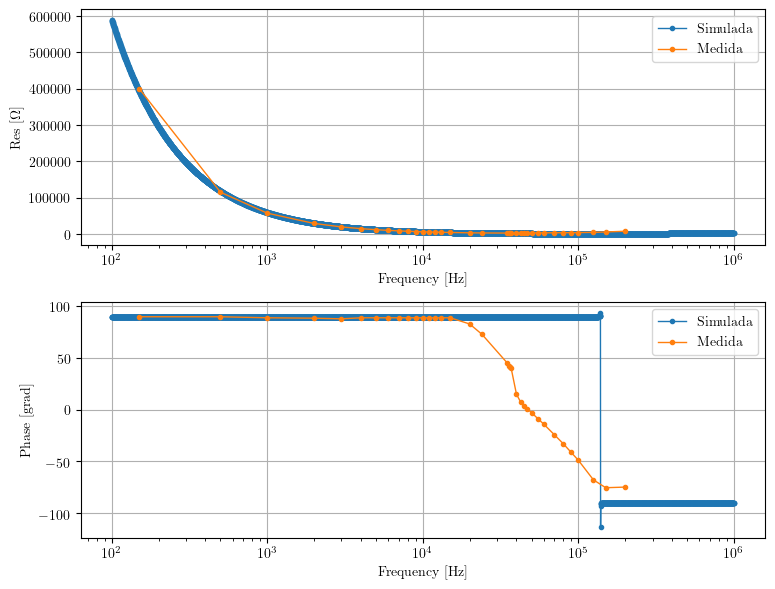
\includegraphics[width=0.8\textwidth]{../Ex4/ZinBodeDERivadorSINcompensarSUPERpuestos.png}}
		\caption{Impedancia de entrada del derivador sin compensar}
		\label{fig:zinsuperDERivador}
	\end{center}
\end{figure}

El valor de las resistencias se logró medir eficazmente pero no se puede decir lo mismo de la fase, esta misma hasta antes de los $20 \, kHz$ coincide con la simulada y tiene una caída de $90º$ a $-90º$ que no es abrupta como en la simulación sino que va bajando durante la década siguiente a $20 \, kHz$.





\section{Circuito Derivador Compensado}
Al presentar el circuito derivador a altas frecuencias un sobrepico con una alta ganancia, se busca tratar de compensarlo de manera tal que no presente este sobrepico.
En este caso se coloca una resistencia en serie al capacitor para compensar el hecho de que a altas frecuencias el capacitor se comporta como un cortocircuito pero teniendo en cuenta que esta no afecte el comportamiento del circuito en las demás frecuencias donde si se tiene el comportamiento deseado.

Para eliminar el sobrepico se eligió un valor de ganancia que en este caso es de $34 \, dB$ y a partir del mismo se calculo la resistencia de compensación ($R_c$) necesaria para tener esta ganancia. El valor de $R_c$ que se obtuvo es de $490 \Omega$ pero se utilizó el valor comercial más cercano que es $470 \Omega$.

\begin{figure}[H]
	\begin{center}
		\makebox[\textwidth]{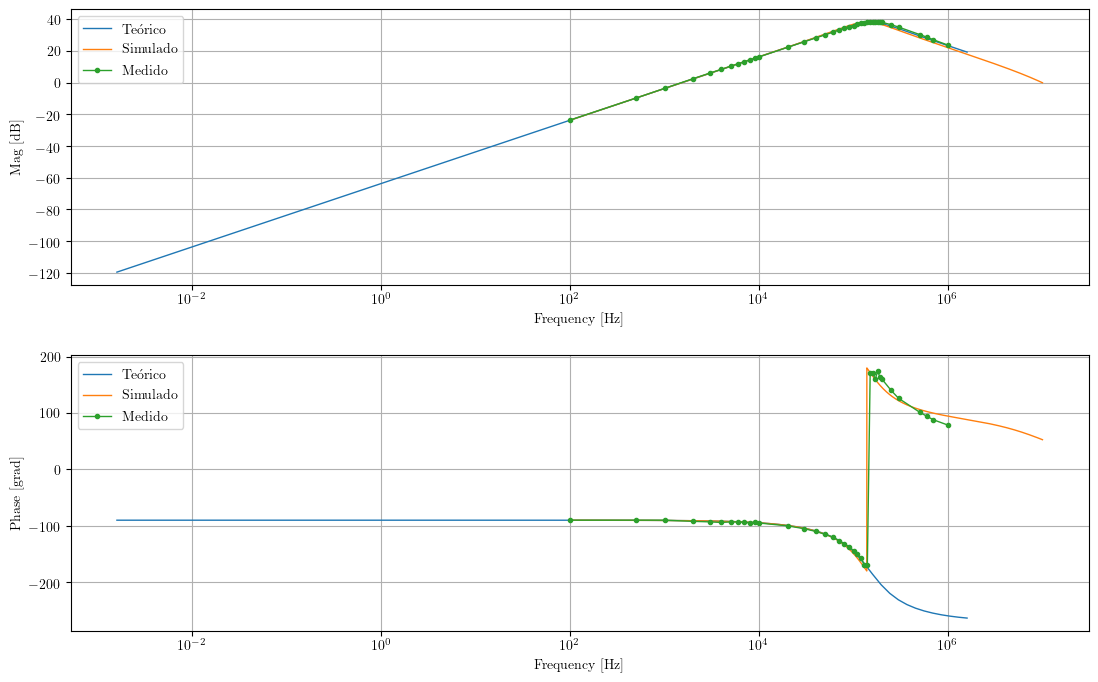
\includegraphics[width=\paperwidth]{../Ex4/BodesSuperpuestosDERivadorCOMPensado.png}}
		\caption{Superposición de bodes para el circuito derivador compensado}
		\label{fig:superposicion3casosderivadorCOMPENSADO}
	\end{center}
\end{figure}

Viendo la Figura \ref{fig:superposicion3casosderivadorCOMPENSADO} se puede notar que el circuito fabricado se comporta de la manera prevista. Esta vez se logró tomar más puntos de medición en las frecuencias cercanas a donde anteriormente se encontraba el sobrepico, pudiendo así decir que se comporta tanto como el simulado y como el teórico en todo el rango de frecuencias medido.

\subsection{Comportamiento ante señales no senoidales}

\begin{figure}[H]
	\begin{center}
		\makebox[\textwidth]{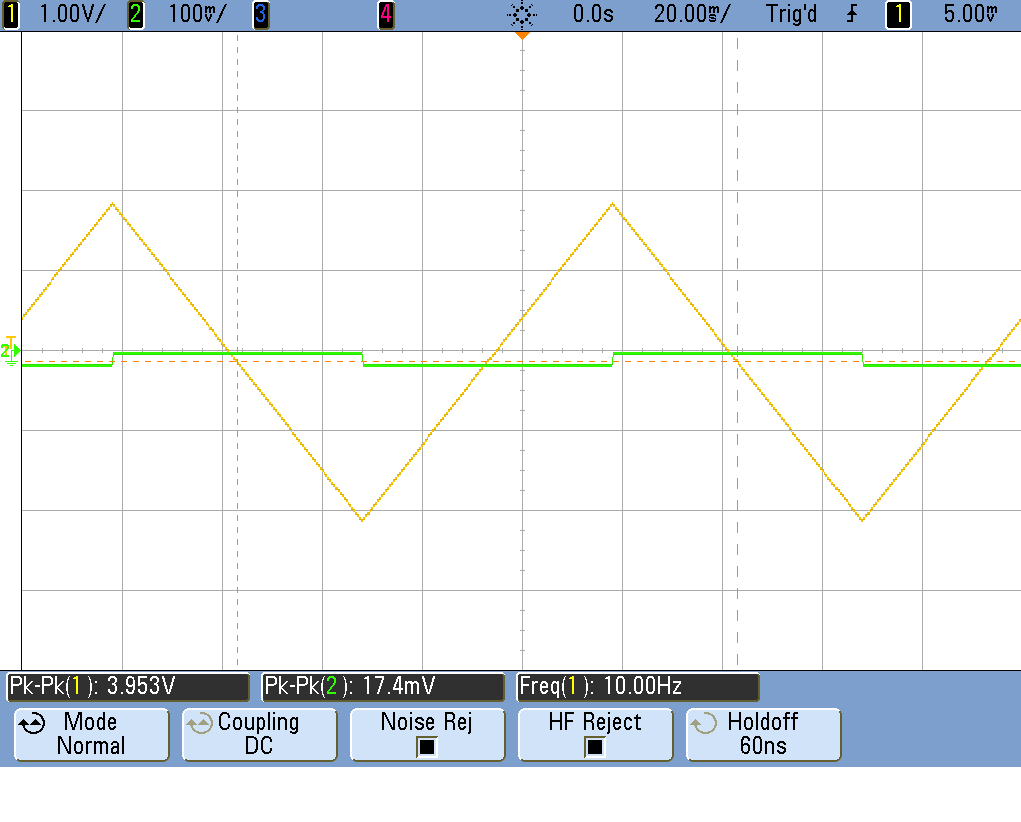
\includegraphics[width=0.8\textwidth]{../Ex4/DerivCOMPTriang10Hz.png}}
		\caption{Derivada de una señal triangular a $10 \,Hz$ - Derivador compensado}
		\label{fig:derivtriangCOMP10Hz}
	\end{center}
\end{figure}

\begin{figure}[H]
	\begin{center}
		\makebox[\textwidth]{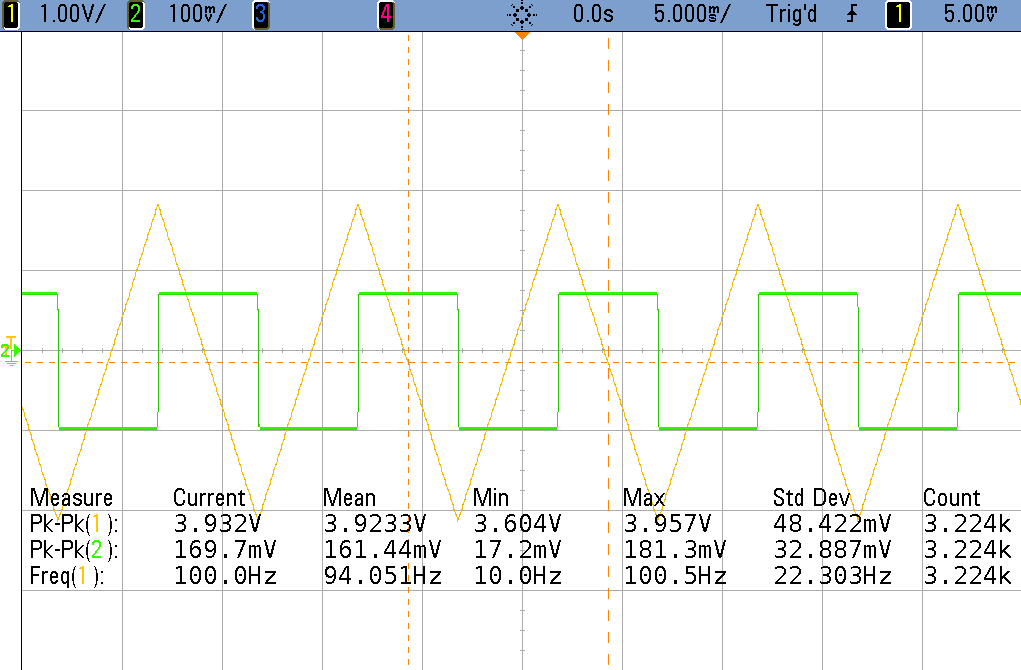
\includegraphics[width=0.7\textwidth]{../Ex4/DerivCOMPTriang100Hz.png}}
		\caption{Derivada de una señal triangular a $100 \,Hz$ - Derivador compensado}
		\label{fig:derivtriangCOMP100Hz}
	\end{center}
\end{figure}

Se puede comprobar gracias a la Figura \ref{fig:derivtriangCOMP10Hz} y \ref{fig:derivtriangCOMP100Hz} que el circuito se sigue comportando de igual manera a frecuencias bajas.

\begin{figure}[H]
	\begin{center}
		\makebox[\textwidth]{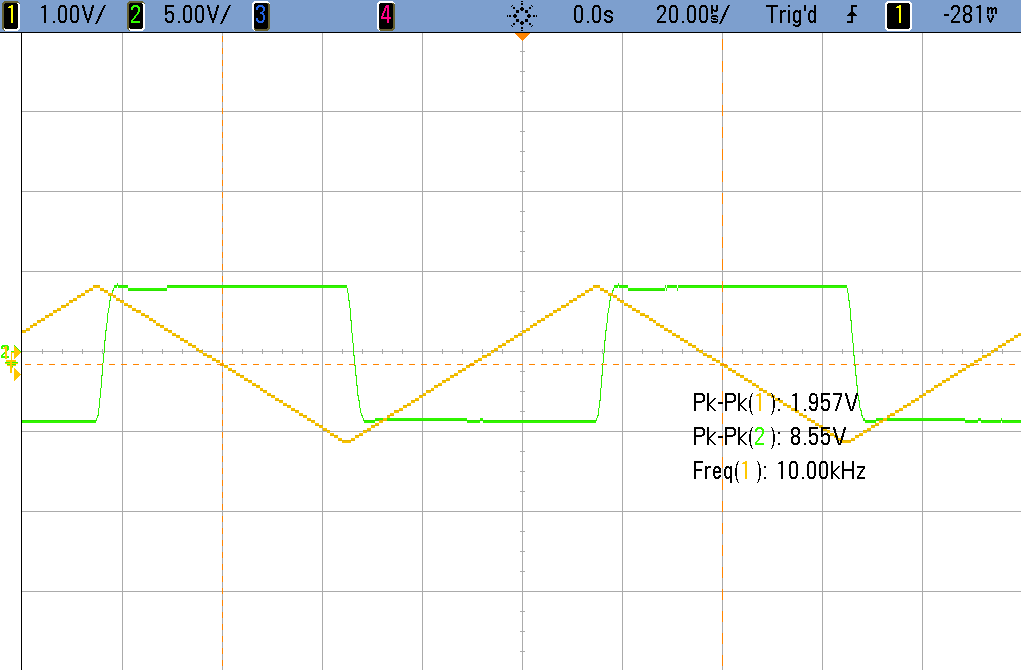
\includegraphics[width=0.7\textwidth]{../Ex4/DerivCOMPTriang10kHz.png}}
		\caption{Derivada de una señal triangular a $10 \,kHz$ - Derivador compensado}
		\label{fig:derivtriangCOMP10kHz}
	\end{center}
\end{figure}

\begin{figure}[H]
	\begin{center}
		\makebox[\textwidth]{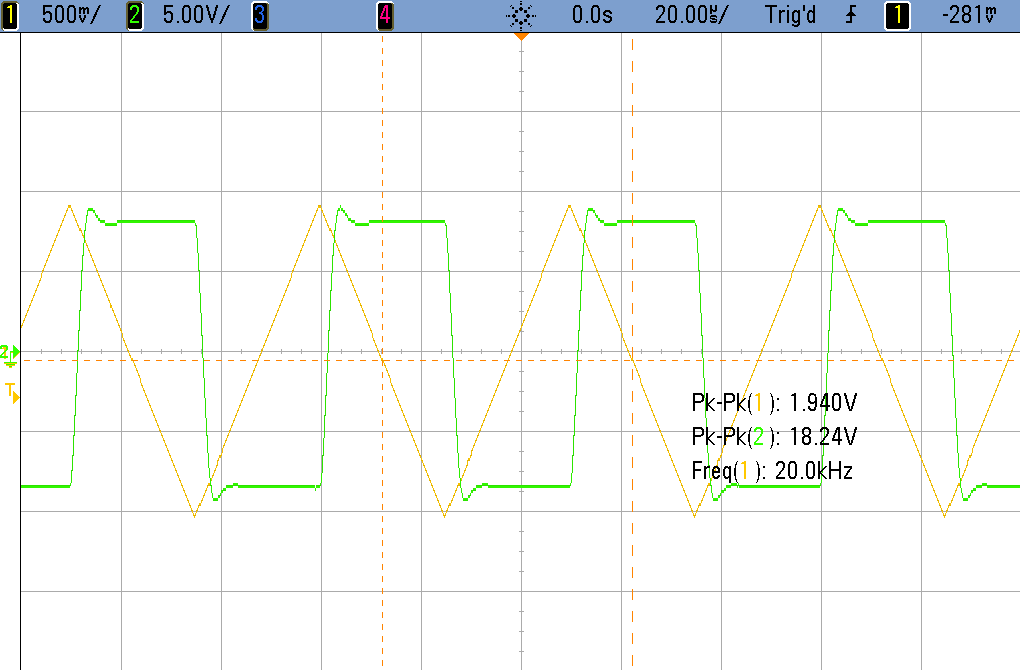
\includegraphics[width=0.7\textwidth]{../Ex4/DerivCOMPTriang20kHz.png}}
		\caption{Derivada de una señal triangular a $10 \,kHz$ - Derivador compensado}
		\label{fig:derivtriangCOMP20kHz}
	\end{center}
\end{figure}

En la Figura \ref{fig:derivtriangCOMP10kHz} y la Figura \ref{fig:derivtriangCOMP20kHz} se puede notar como a estas frecuencias la salida es una señal cuadrada que se estabiliza más rápido que las vistas en la Figura \ref{fig:derivtriangNOcomp10kHz} y Figura \ref{fig:derivtriangNOcomp20kHz}.

\begin{figure}[H]
	\begin{center}
		\makebox[\textwidth]{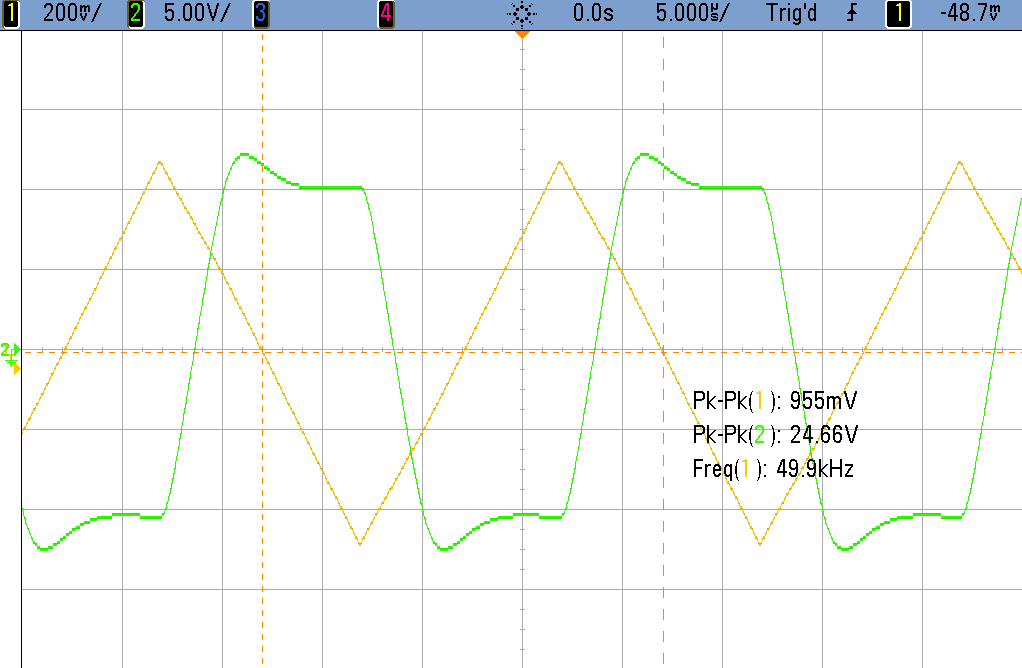
\includegraphics[width=0.7\textwidth]{../Ex4/DerivCOMPTriang50kHz.png}}
		\caption{Derivada de una señal triangular a $50 \,kHz$ - Derivador compensado}
		\label{fig:derivtriangCOMP50kHz}
	\end{center}
\end{figure}

A $50 \, kHz$ el circuito sigue cumpliendo con su función de derivar, a diferencia del circuito derivador sin compensar que a los $20 \, kHz$ no nos entregaba una señal cuadrada ya que no tenía el tiempo suficiente para estabilizarse.

\begin{figure}[H]
	\begin{center}
		\makebox[\textwidth]{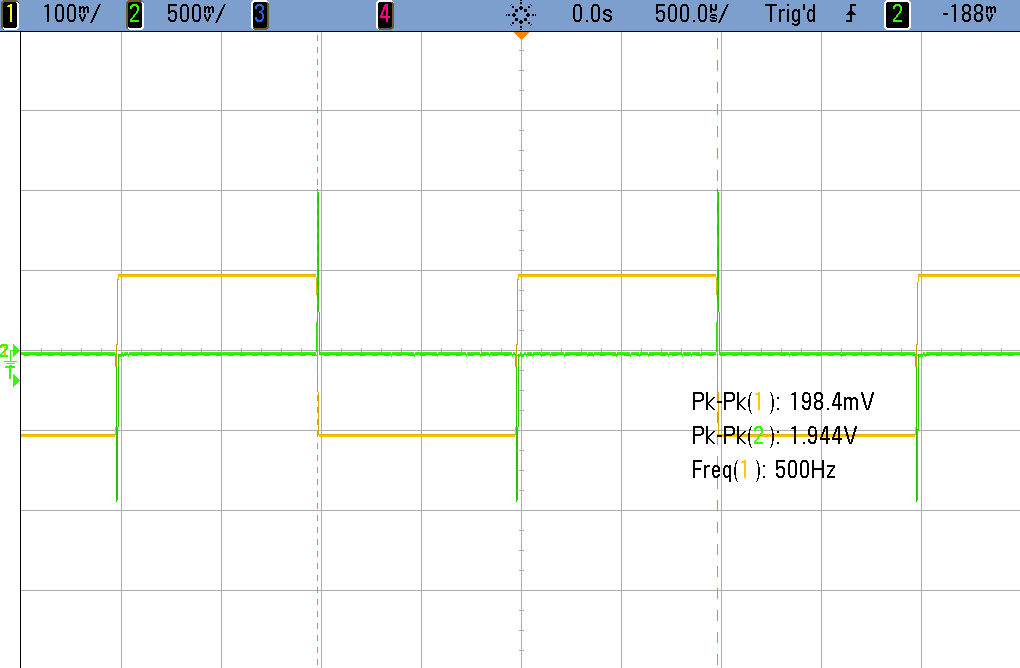
\includegraphics[width=0.7\textwidth]{../Ex4/DerivCOMPCuadrada.png}}
		\caption{Derivada de una señal cuadrada a $500 \,Hz$ - Derivador compensado}
		\label{fig:derivCUAdradaCOMP}
	\end{center}
\end{figure}

Ahora también es apreciable la derivada de una señal cuadrada la cual son pulsos, como puede verse en la Figura \ref{fig:derivCUAdradaCOMP}.

\subsection{Impedancia de entrada}
\begin{figure}[H]
	\begin{center}
		\makebox[\textwidth]{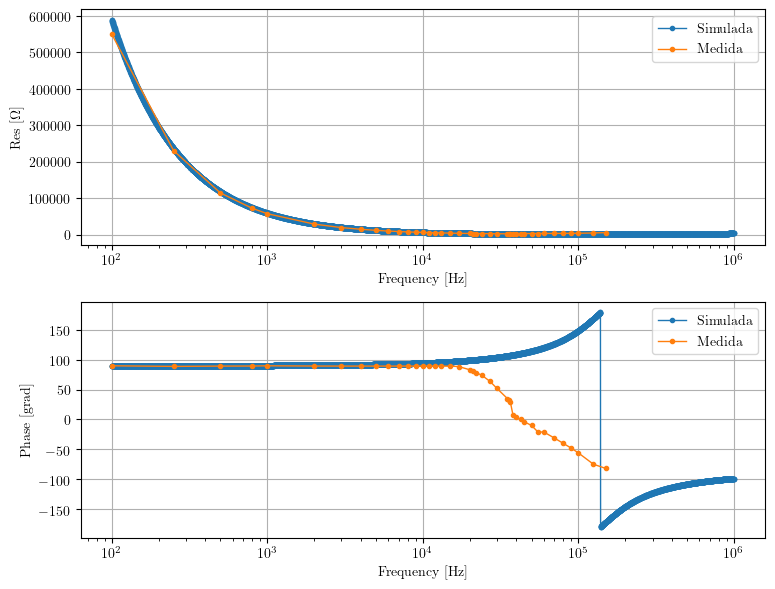
\includegraphics[width=0.8\textwidth]{../Ex4/ZinBodeDERivadorCOMpensadoSUPERpuestos.png}}
		\caption{Impedancia de entrada del derivador compensado}
		\label{fig:zinsuperDERivadorCompensado}
	\end{center}
\end{figure}

Similar al caso anterior, el valor de la impedancia de entrada logro medirse de forma eficaz mientras que la fase sigue siendo válida pero sólo para frecuencias menores a $20 \, kHz$.








\section{Circuito Integrador}
En este caso al circuito visto en la Figura \ref{fig:circconz1z2} se le reemplazo $Z_2$ por un capacitor y $Z_1$ por una resistencia como puede verse en la Figura \ref{fig:circuitointegrador}. En este caso $Z_2=\dfrac{1}{s \, C}$ y $Z_1= R$.

\begin{figure}[H]
\centering
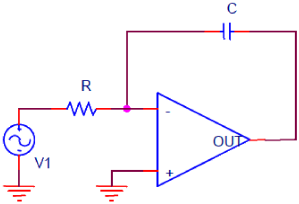
\includegraphics[scale=0.5]{../Ex4/circuitointegrador.png}
\caption{Circuito integrador}
\label{fig:circuitointegrador}
\end{figure}

Utilizando también para este caso $\mathrm{A_{vol}}=110$.

\subsection{Ganancia ideal} \label{gananciaidealintegrador}
Para este caso se obtiene:

\begin{equation}
G_I=-\dfrac{1}{C\,R\,S}
\end{equation}

\begin{center}
	\begin{figure}[H]	
	\makebox[\textwidth]{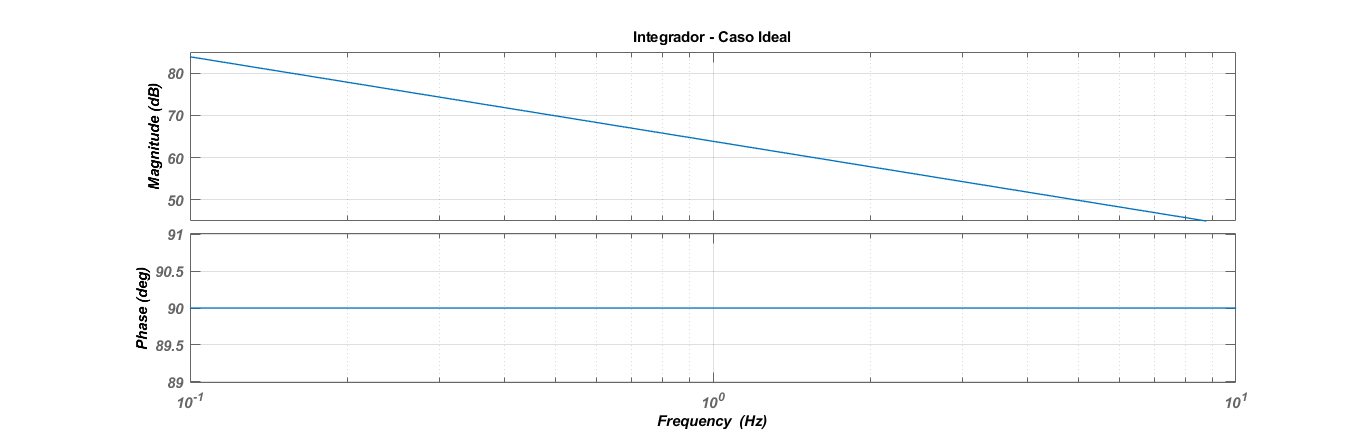
\includegraphics[width=\paperwidth]{../Ex4/Integrador-CasoIdeal.png}}
	\caption{Ganancia para el caso ideal del integrador}
	\label{fig:avolidealintegrador}
	\end{figure}
\end{center}

Si se realiza la antitransformada recordando que $H(s)= \dfrac{V_{out}}{V_{in}}$ obtenemos:
\begin{equation} 
v_{out} (t) = - \, \dfrac{1}{R \,C} \,  \int_{\infty}^t v_{in}(u) du
\end{equation}

Donde se observa que la función a la salida es la integral de la función a la entrada multiplicada por una constante que es $- \, \dfrac{1}{R \,C}$. También al observar la función transferencia se puede notar un desfasaje de $90º$ y la presencia de un polo simple en $f \sim 1.5 \,kHz$, lo que otorga una atenuación de $20 \, dB$ por década, entonces a altas frecuencias la tensión de salida tiende a $0 \,V$. 
También es importante notar que para este caso la ganancia de una corriente continua es infinita.

\subsection{$\mathrm{A_{vol}}$ finito}
\begin{equation}
H(s)=- \dfrac{\mathrm{A_{vol}}}{C\,s\,\left(R\,\left(\mathrm{A_{vol}}+1 \right) + \frac{1}{C\,S}\right)} = -\dfrac{\mathrm{A_{vol}}}{R\,C\,\left( \mathrm{A_{vol}} + 1 \right)\,s + 1}
\end{equation}

En este caso el polo se encuentra ahora en $f \sim 5 \, mHz$, como puede verse en la Figura \ref{avolfinitointegrador} y la fase comienza en $180º$ y cae hasta $90º$.

\begin{figure}[H]
	\begin{center}
		\makebox[\textwidth]{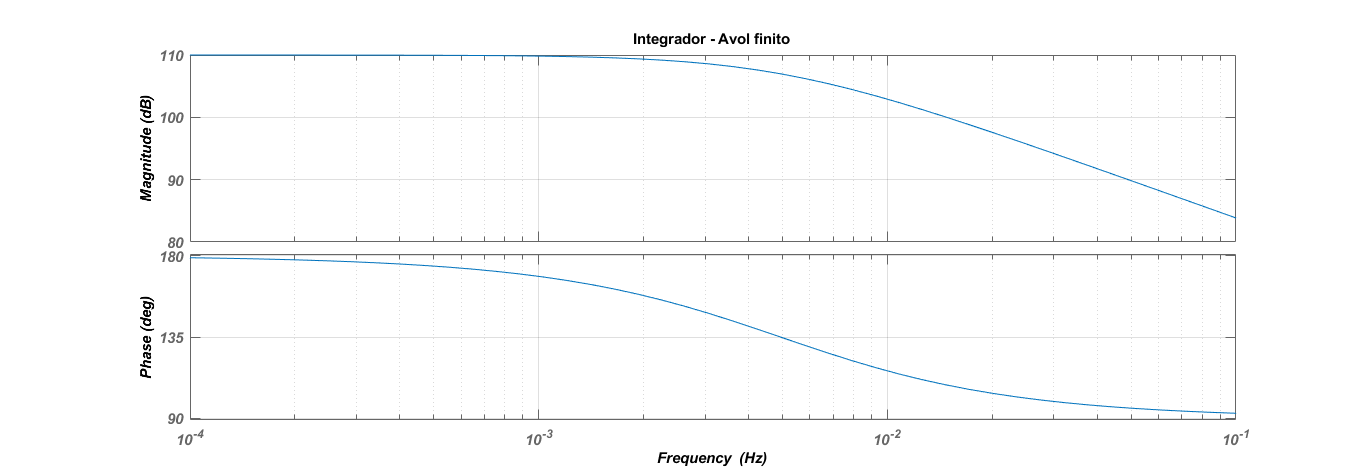
\includegraphics[width=\paperwidth]{../Ex4/Integrador-AvolfinitoBodeAutomatico.png}}
		\caption{Ganancia para el caso con $A_{vol}$ finito del integrador}
		\label{avolfinitointegrador}
	\end{center}
\end{figure}

\subsection{$\mathrm{A{vol}(w)}$ con polo dominante}
\begin{equation}
H(s)= -\frac{\mathrm{A_{vol}}}{C\,s\,\left(\frac{s}{\mathrm{w_p}}+1\right)\,\left(\dfrac{1}{C\,s}+R\,\left(\dfrac{\mathrm{A_{vol}}}{\dfrac{s}{\mathrm{w_p}}+1}+1\right)\right)}
= - \dfrac{\mathrm{A_{vol}}}{C\,R\,s^2+(C\,R\,w_p+C\,R\,w_p\,\mathrm{A_{vol}}+1)s+w_p}
\end{equation}

\begin{figure}[H]
	\begin{center}
		\makebox[\textwidth]{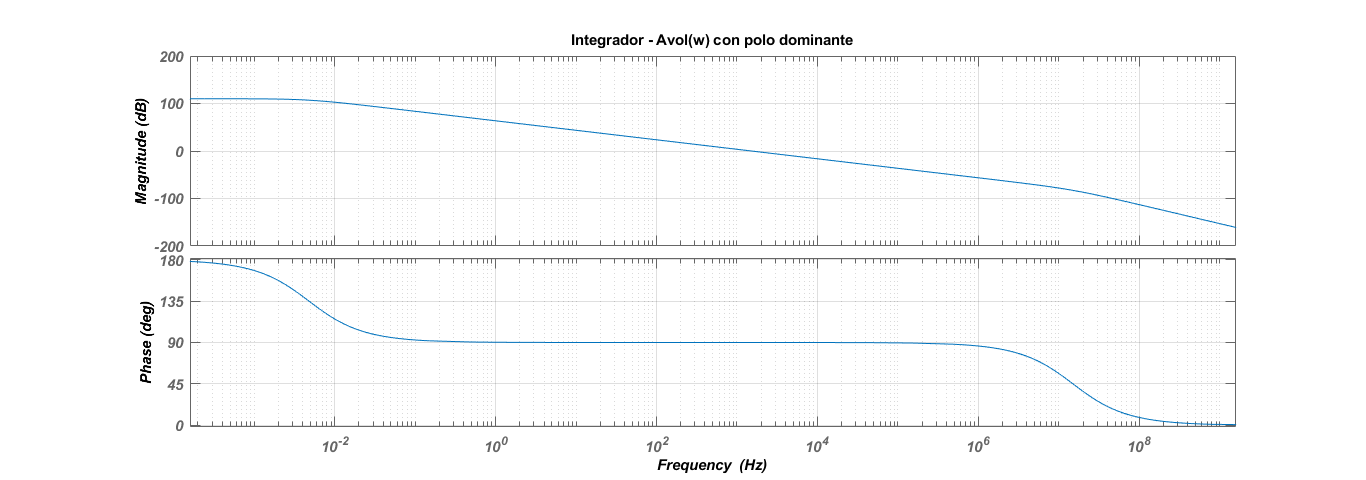
\includegraphics[width=\paperwidth]{../Ex4/Integrador-Avol(w)conpolodominanteHasta11MHz.png}}
		\caption{Ganancia para el caso con $A_{vol}(w)$ con polo dominante del integrador}
		\label{avolpolodominanteintegrador}
	\end{center}
\end{figure}

En este caso se tienen dos polos simples en $f \sim 5 \, mHz$ y $f \sim 15 \, MHz$ pero en ninguno de ellos es posible medir ya que en el primer caso la frecuencia es muy pequeña y tiene una ganancia de $110 \, dB$ y en el otro caso la atenuación es tanta que necesitaríamos más de los $20 V_{pp}$ que nos puede ofrecer el instrumental del laboratorio para poder medir.

\subsection{Comparación de los 3 casos}
\begin{figure}[H]
	\begin{center}
		\makebox[\textwidth]{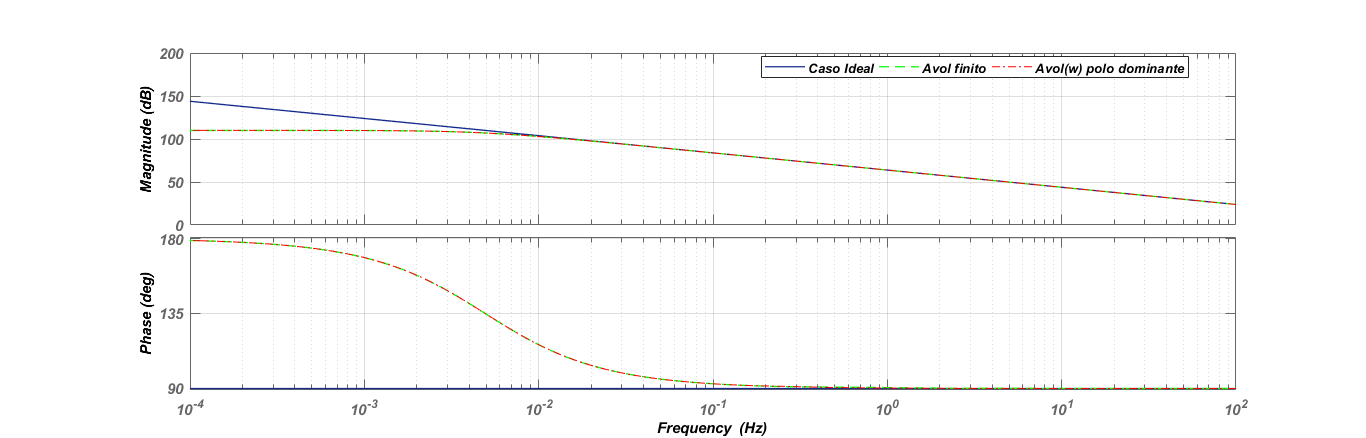
\includegraphics[width=\paperwidth]{../Ex4/BodesSuperpuestosIntegrador.png}}
		\caption{Superposición de los tres casos}
		\label{fig:comparacion3avolintegrador}
	\end{center}
\end{figure}

Viendo el gráfico se notó que a frecuencias mayores a $1 \, Hz$ tanto la amplitud como la fase de las tres funciones se comportan de forma idéntica, por lo que si se trabaja con frecuencias mayores a $1 \, Hz$ el circuito debe cumplir con el propósito de su diseño, el de integrar.

\subsection{Medición vs. simulación vs. teórico}
\begin{figure}[H]
	\begin{center}
		\makebox[\textwidth]{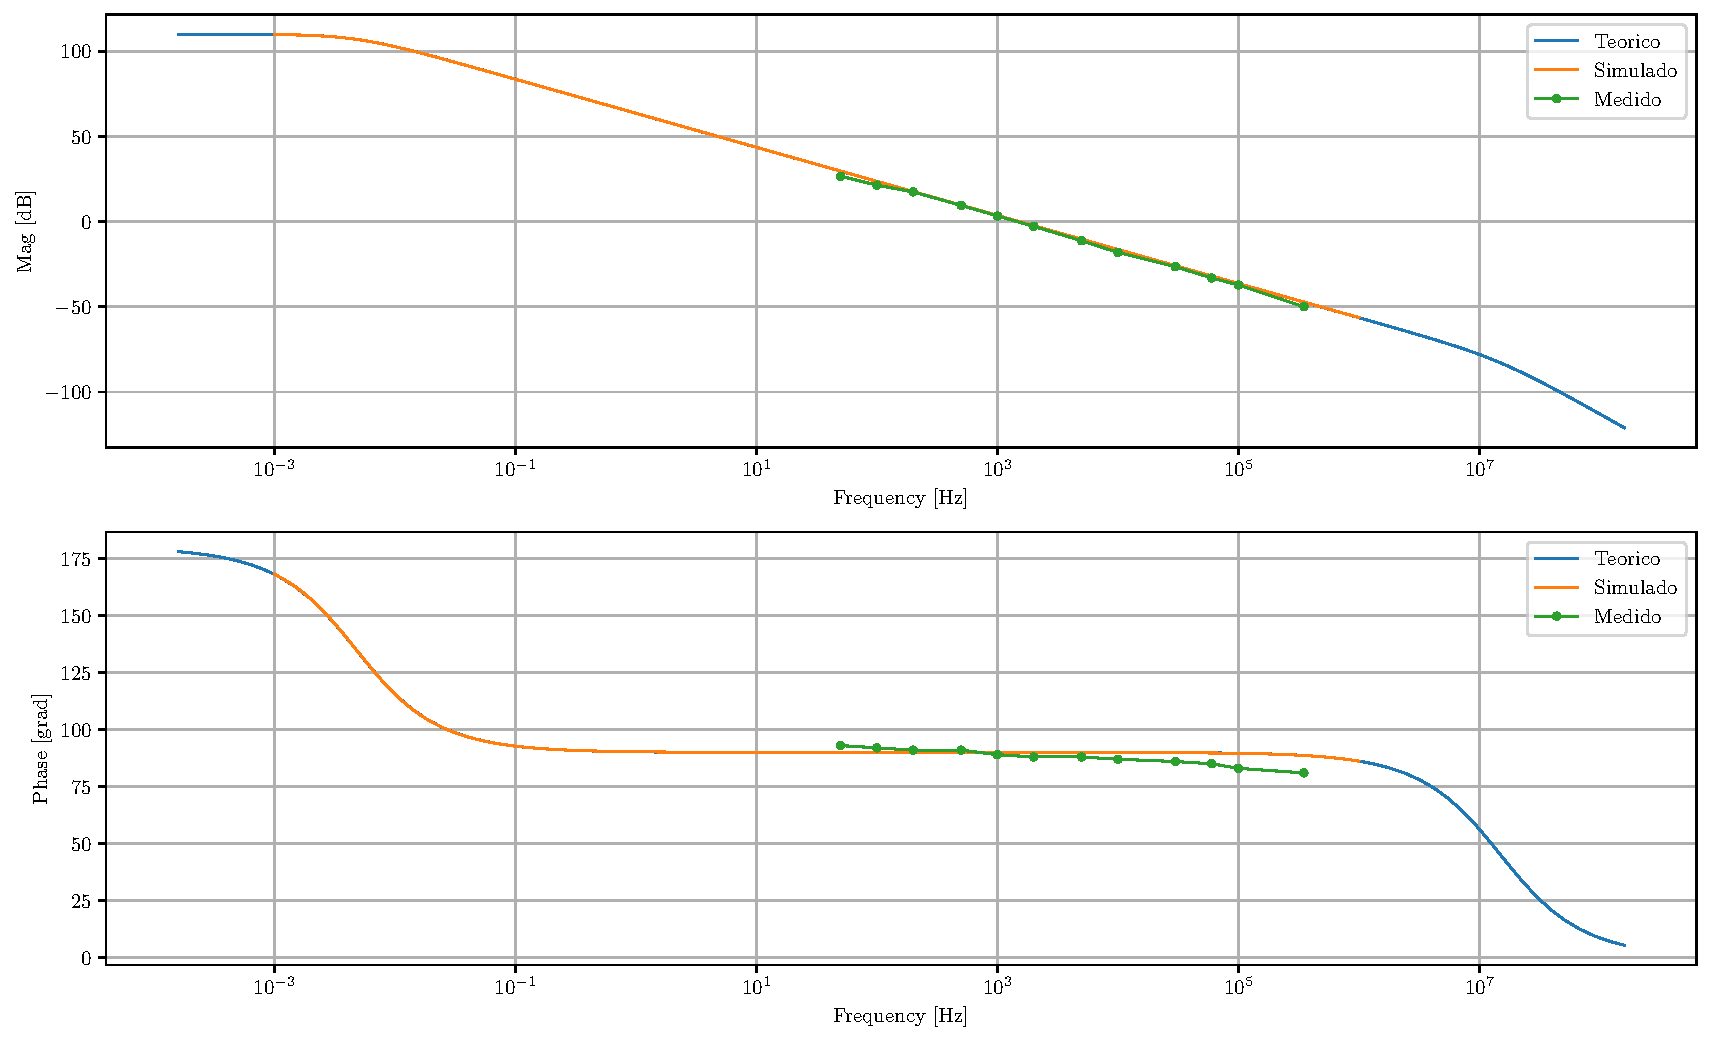
\includegraphics[width=\paperwidth]{../Ex4/BodesSuperpuestosINTegradorSINCOMPensar.pdf}}
		\caption{Superposición de bodes para el circuito integrador}
		\label{fig:superposiciontrescasosINTegrador}
	\end{center}
\end{figure}

En los rangos de frecuencia en los que se pudo medir la respuesta en frecuencia sin que la señal de salida se viera saturada al amplificarse o se viera sumamente atenuada se comprobó que el circuito integrador se comporto como se esperaba, fue una tarea complicada el medir debido a que como se menciono anteriormente en la Sección \ref{gananciaidealintegrador} las señales de continua se veían amplificadas al infinito, por lo que cualquier mínima señal de continua hacía que la señal medida se encontrará en el valor de $V{cc-}$ de alimentación del amplificador operacional.

\subsection{Comportamiento ante señales no senoidales}

\begin{figure}[H]
	\begin{center}
		\makebox[\textwidth]{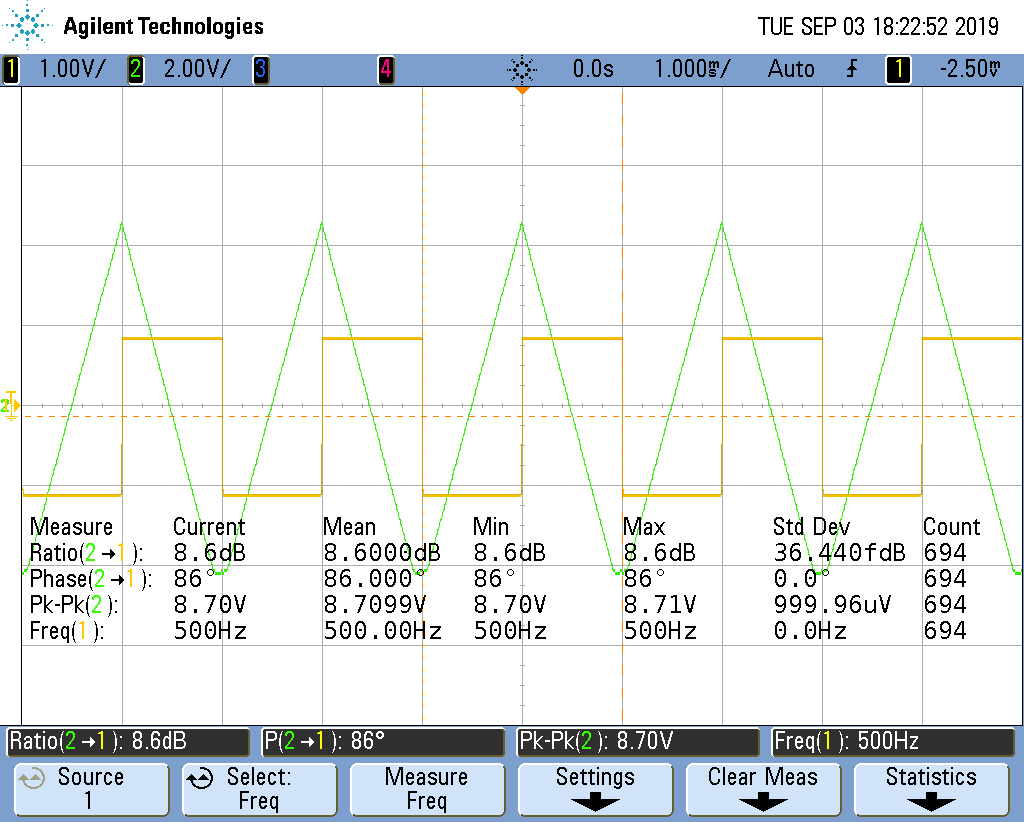
\includegraphics[width=0.8\textwidth]{../Ex4/Integrador500Hz.png}}
		\caption{Integral de una señal cuadrada a $500 \, Hz$}
		\label{fig:IntegralNOcomp500Hz}
	\end{center}
\end{figure}

\begin{figure}[H]
	\begin{center}
		\makebox[\textwidth]{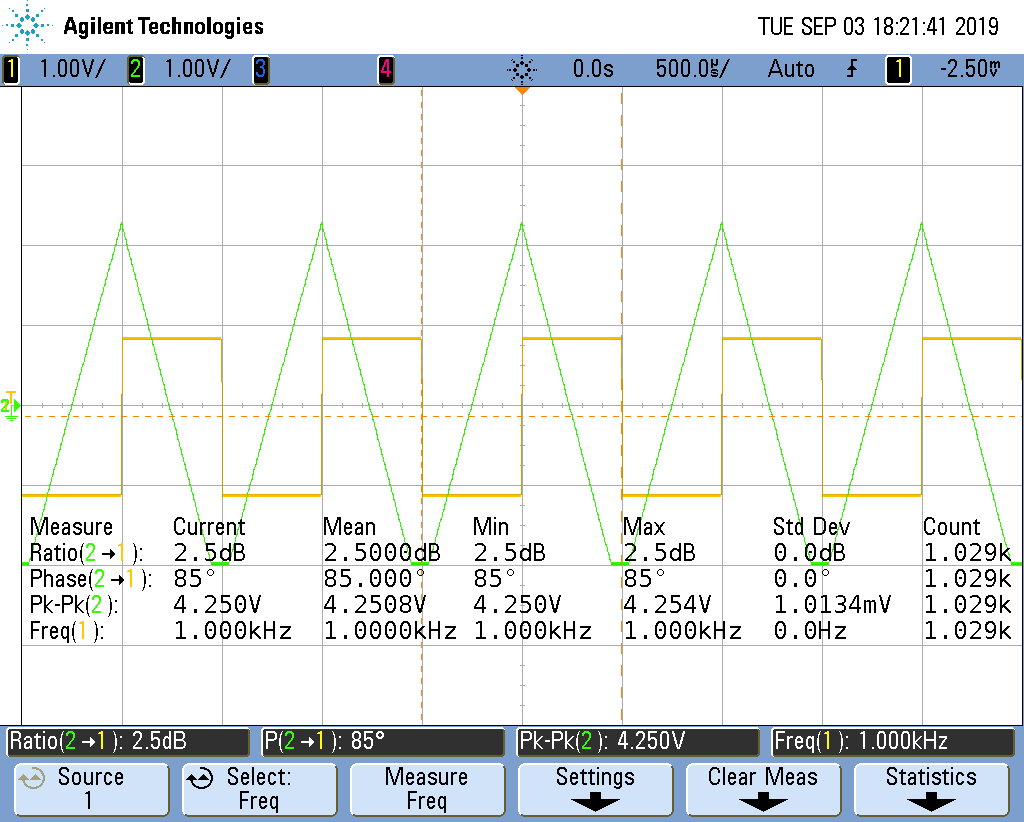
\includegraphics[width=0.8\textwidth]{../Ex4/Integrador1kHz.png}}
		\caption{Integral de una señal cuadrada $1 \, kHz$}
		\label{fig:IntegralNOcomp1kHz}
	\end{center}
\end{figure}

Observando la Figura \ref{fig:IntegralNOcomp500Hz} y la Figura \ref{fig:IntegralNOcomp1kHz} se puede ver que a frecuencias bajas el integrador se encuentra cumpliendo su propósito ya que está integrando la señal de entrada cuadrada amarilla en una señal triangular en la señal de salida. Notar que la amplitud de la tension de entrada es de $2 \, V_{pp}$ y que la de la señal de salida en $500 \,Hz$ es de $8,7 \,V$ y la de $1 \,kHz$ es de $4,25 \,$, pudiendo así notar como la amplitud de la señal de salida va disminuyendo a medida que la frecuencia de la señal de entrada es más alta.

\subsection{Impedancia de entrada}
\begin{figure}[H]
	\begin{center}
		\makebox[\textwidth]{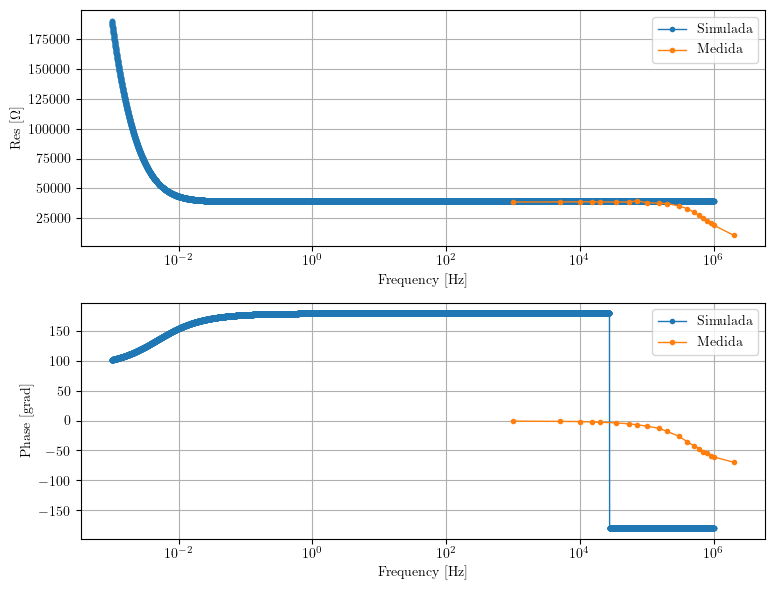
\includegraphics[width=0.8\textwidth]{../Ex4/ZinBodeINTegraadorCOMpensadoSUPERpuestos.png}}
		\caption{Impedancia de entrada del integrador sin compensar}
		\label{fig:zinsuperINTegrador}
	\end{center}
\end{figure}

En este caso mientras el valor de la impedancia de entrada coincide hasta apróximadamente $400 \, kHz$ la fase no coincide en ningún punto.


\section{Circuito Integrador Compensado}
El circuito integrador presenta una ganancia infinita a frecuencias bajas y una atenuación muy grande que crece rápidamente a medida que aumenta la frecuencia.

En este caso se coloca una resistencia en paralelo al capacitor para compensar el hecho de que a bajas frecuencias el capacitor se comporta como un circuito abierto y entonces el sistema deja de estar retroalimentado. No se debe olvidar para este caso también que la resistencia que se elige debe ser tal que no afecte el comportamiento del circuito en las frecuencias donde si se tiene el comportamiento deseado.

Similar al caso del circuito derivador compensado se eligió un valor de ganancia que en este caso es de $20 \, dB$ y a partir del mismo se calculo la resistencia de compensación ($R_c$) necesaria para tener esta ganancia. El valor de $R_c$ que se obtuvo es de $39 \,k \Omega$.

\begin{figure}[H]
	\begin{center}
		\makebox[\textwidth]{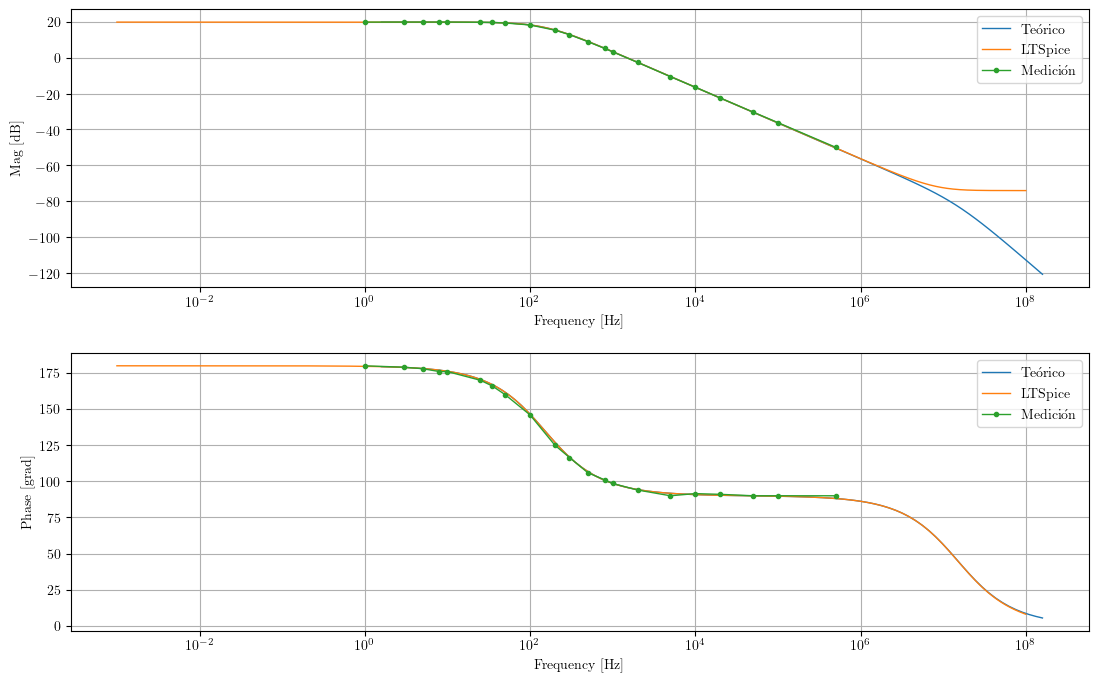
\includegraphics[width=\paperwidth]{../Ex4/BodesSuperpuestosINTegradorCOMPensado.png}}
		\caption{Superposición de bodes para el circuito integrador compensado}
		\label{fig:superposicion3casosintegradorCOMPENSADO}
	\end{center}
\end{figure}

Viendo la Figura \ref{fig:superposicion3casosintegradorCOMPENSADO} se puede notar que el circuito fabricado se comporta de la manera prevista. Esta vez no existieron los problemas de saturación debido a alguna coriente continua por mínima que sea y se logró una mejor medición. Se puede decir que se comporta tanto como el simulado y como el teórico en todo el rango de frecuencias medido.

\subsection{Comportamiento ante señales no senoidales}

\begin{figure}[H]
	\begin{center}
		\makebox[\textwidth]{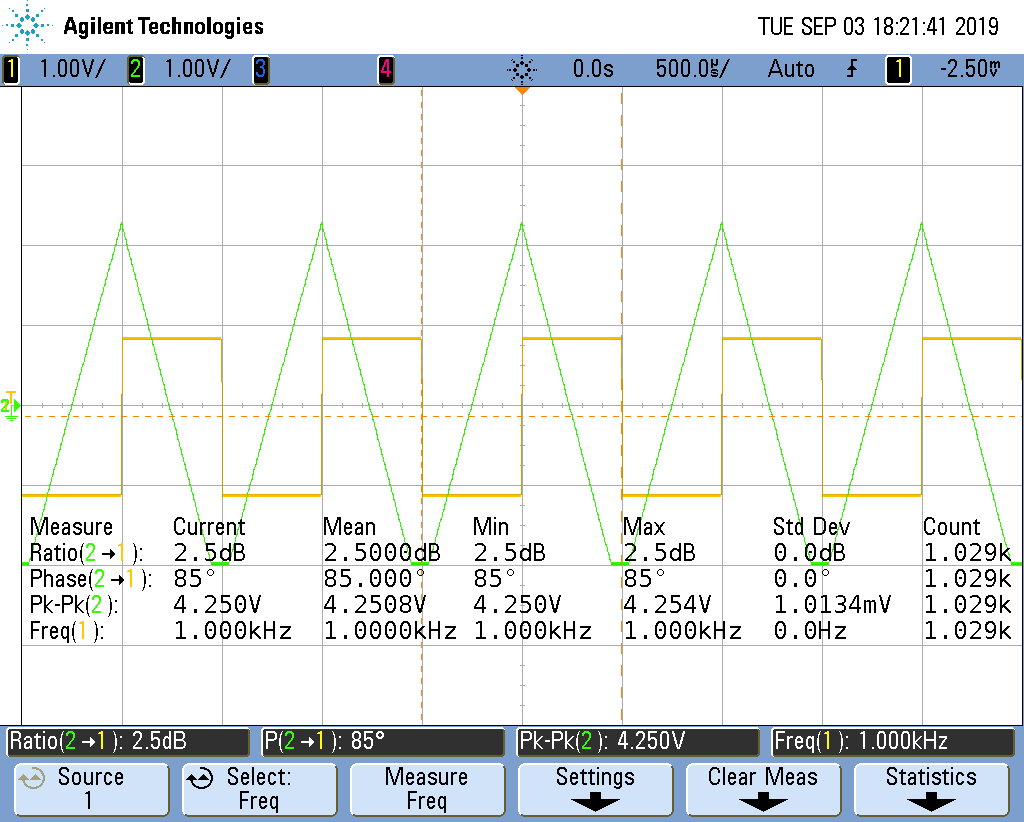
\includegraphics[width=0.8\textwidth]{../Ex4/Integrador1kHz.png}}
		\caption{Integral de una señal cuadrada a $1 \, Hz$}
		\label{fig:IntegralCOMP1Hz}
	\end{center}
\end{figure}

Se puede observar que el circuito a la frecuencia de $1 \, Hz$ no se encuentra cumpliendo su función de integrar, pero si volvemos a la Figura \ref{fig:superposicion3casosintegradorCOMPENSADO} se logra ver que el circuito sólo debe amplificar la señal de entrada de $2 \, V_{pp}$ a casi $20 V_{pp}$, en esta frecuencia.

\begin{figure}[H]
	\begin{center}
		\makebox[\textwidth]{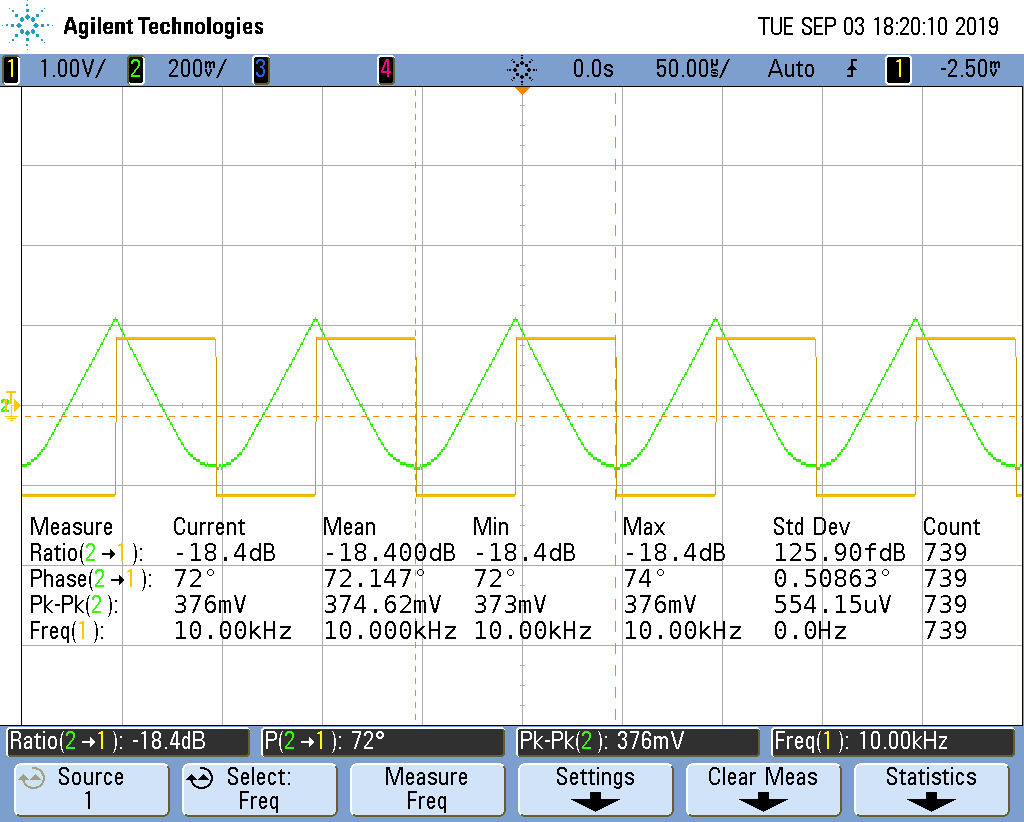
\includegraphics[width=0.8\textwidth]{../Ex4/Integrador10kHz.png}}
		\caption{Integral de una señal cuadrada $10 \, kHz$}
		\label{fig:IntegralCOMP10kHz}
	\end{center}
\end{figure}

A $10 \, kHz$ de frecuencia es posible ver como con la señal cuadrada amarilla que es la señal de entrada del circuito se obtiene la señal triangular verde que sería la señal integrada y multiplicada por aquel factor negativo como se vio en el caso anterior del derivador.

\subsection{Impedancia de entrada}
La impedancia de entrada en este caso da un valor constante de $39 \, k \Omega$ y una fase de $180º$.

\section{Conclusión}
Se logró diseñar los circuitos pedidos que derivan o integran señales en un rango de frecuencias determinado, se conocieron sus limitaciones debido a comportamientos no deseados y se busco la forma de compensarlos para poder tener un mejor rango de frecuencias en el cual poder utilizarlos.
